%% The following is a directive for TeXShop to indicate the main file
%%!TEX root = diss.tex

\chapter{Identification of Germline Alterations in FFPE Tumours}
\label{ch:IdentificationofGermlineAlterationsinFFPETumours}

Tumour-only sequencing is commonly performed by clinical laboratories to detect targetable somatic mutations, which facilitate treatment with molecularly targeted drugs. Unlike the research setting, matched normal samples such as blood, saliva, or adjacent normal tissues are not routinely processed in the clinical setting due to limited sample availability, funding, and time. The tumour genome also contains germline information that may have clinical implications for patients and their families. For instance, germline alterations in cancer-predisposing genes could facilitate implementation of cancer preventative measures such as early screening and routine surveillance. Moreover, germline PGx variants could predict response to drugs like chemotherapeutic agents, thereby preventing adverse drug reactions.

Because the tumour genome consists of both germline and somatic alterations, it is important to establish approaches to distinguish between germline and somatic alterations in cancer diagnostic assays that only sequence tumour DNA. In the absence of matched normal samples, approaches such as constructing a virtual normal from a combination of variants identified in multiple normal samples from healthy individuals and filtering variants using public databases such as such as dbSNP, 1000 Genomes Project, and COSMIC could enable the differentiation of germline variations from somatic mutations. Subsequently, potential germline alterations can be referred to follow-up testing, which involves genetic counseling and collection of germline samples for further sequencing and analysis.

The TOP study is comprised of 213 patients with tumour and matched blood specimens. We interpreted the germline variants identified in blood specimens from TOP patients using the effect prediction software, SnpEff (version 4.2), and ExAC and 1000 Genomes databases, which provide information on population frequency. We also annotated the variant calls with the ClinVar database, which enable assessment of clinical significance, Furthermore, we performed manual literature review to determine the functional and clinical impacts of all germline alterations detected in the blood samples. Because several studies demonstrated that a germline cancer-predisposing variant is present in 3-10\% of patients undergoing tumour-normal sequencing \cite{Raymond2016,Meric-Bernstam2016,Schrader2015,Jones2015}, we sought to confirm the presence of germline alterations in the tumour genome by measuring variant concordance between blood and tumour DNA.

Lastly, we differentiated between germline and somatic statuses of variants identified in tumour DNA through applying VAF thresholds. While heterozygous germline variants are expected to have VAF of close to 50\%, homozygous germline variants are expected to have VAF of close to 100\%. In contrast, the VAF of somatic mutations relies on tumour content. Due to contamination of normal tissues in tumour biopsies, it is highly likely that the VAFs of somatic mutations are substantially lower than the expected VAFs for germline alterations. As we have matched blood samples for all tumour samples, we were able to evaluate the sensitivity of using VAF thresholds to discriminate between germline and somatic alterations in tumour DNA. Furthermore, we also assessed the positive predictive value of referring potential germline alterations for follow-up testing. Through this analysis, we hope to establish a VAF cut-off that could maximize true positive rate for identification of germline alterations from tumour-only analyses, as well as minimize false positive rate to reduce unnecessary follow-up testing, which could cause patients avoidable psychological distress and hassles.

Together, our analyses would provide insights on whether application VAF threshold is a practical approach to distinguish between germline and somatic alterations in tumour-only sequencing assays. Hence, this will determine whether tumour-only sequencing assays can be leveraged by clinical laboratories for initial screening of germline alterations that are clinically relevant.

%%%%%%%%%%%%%%%%%%%%%%%%%%%%%%%%%%%%%%%%%%%%%%%%%%%%%%%%%%%%%%%%%%%%%
\section{Frequency and variant assessment of germline alterations in patients from TOP cohort}
\label{sec:FrequencyandvariantassessmentofgermlinealterationsinpatientsfromTOPcohort}
%%%%%%%%%%%%%%%%%%%%%%%%%%%%%%%%%%%%%%%%%%%%%%%%%%%%%%%%%%%%%%%%%%%%%

We examined 15 cancer-related genes and six PGx genes in DNA isolated from blood samples from the 213 cancer patients in TOP cohort. We identified a total of 1990 germline alterations that passed our filtering criteria (\autoref{fig:variant_pipeline}B). In 212 out of 213 patients, we detected a total of 1205 variants in the 15 cancer-related genes screened by the OncoPanel, with an average of 5.7 variants per patient (standard error = 0.15, range = 1--11 variants; \autoref{tbl:freq_cancer_genes}). These germline alterations were found at 50 genomic positions and interpreted using various bioinformatics approaches and literature review (\autoref{tbl:germline_cancer_genes}). Through effect prediction using the SnpEff software, we demonstrated that 78\% of these variants were synonymous, 16\% were missense variants, 4\% occurred within splice regions, and 2\% were frameshift variants. Eighteen out of the 50 germline variants were classified as common variants by the 1000 Genomes Project with population frequencies of $\geq$ 1\% in the ExAC database, whereas eight out of the 50 variants were classified as rare variants with population frequencies of $<$ 1\% in the ExAC database.

To assess clinical significance of the 50 germline alterations in cancer-related genes, we used information in the ClinVar database. Our assessment revealed 16\% benign variants, 16\% likely benign variants, 12\% annotated as benign/likely benign, 4\% with conflicting interpretations of pathogenicity, and 2\% with uncertain significance. We were unable to determine the clinical significance of 48\% of the 50 germline variants because these variants were not reported in the ClinVar database. While we found no variants that were pathogenic or likely pathogenic, we identified one TP53 variant, p.Arg72Pro$/$c.215G$>$C (rs1042522), that is associated with drug response. Based on literature review, clinical studies revealed that the Pro/Pro genotype results in severe neutropenia in ovarian cancer patients receiving cisplatin-based chemotherapy, and poor survival and treatment response in gastric cancer patients receiving paclitaxel and capecitabine combination chemotherapy, as well as 5-fluorouracil-based adjuvant chemotherapy. The combination of evidence from our literature review and the ClinVar database suggests that the TP53 p.Arg72Pro$/$c.215G$>$C (rs1042522) could be potentially useful in guiding therapeutic intervention for cancer patients.

Furthermore, we identified a total of 785 variants in the six PGx genes screened by the OncoPanel in 212 out of 213 patients, with an average of 3.7 germline alterations per patient (standard error = 0.10, range = 1--8 variants; \autoref{tbl:freq_germline_pgx_genes}). These PGx variants occurred at 23 genomic positions and were interpreted using similar methods to the germline alterations identified in cancer-related genes (\autoref{tbl:germline_pgx_genes}). Effect prediction using the SnpEff software demonstrated that 57\% of these 23 germline variants were missense variants, 17\% were synonymous, 9\% occurred within splice regions, 9\% occurred upstream of a gene, 4\% were located at splice donor sites, and 4\% were present at the 3' untranslated region. Ten out of the 23 germline variants were classified as common variants by the 1000 Genomes Project with population frequencies of $\geq$ 1\% in the ExAC database, whereas one out of the 23 variants was classified as a rare variant with population frequency of $<$ 1\% in the ExAC database.

We also assessed clinical significance of the germline alterations in the PGx genes using the ClinVar database. This assessment demonstrated that 21\% of the 23 variants were categorized as either benign or likely benign, 17\% with conflicting interpretations of pathogenicity, 9\% submitted without assessment of clinical significance, and 4\% with uncertain significance. There was also 17\% of variants that were not reported in the ClinVar database. Although our analysis showed no variants that were pathogenic or likely pathogenic in the PGx genes, we identified seven out of the 23 germline alterations that were associated with drug response. These alterations are DPYD p.Asp949Val$/$c.2846A$>$T (rs67376798), c.1906G$>$A (rs3918290), p.Met166Val$/$c.496A$>$G (rs2297595), GSTP1 p.Ile105Val$/$c.313A$>$G (rs1695), MTHFR p.Glu429Ala$/$c.1286A$>$C (rs1801131), p.Ala222Val$/$c.665C$>$T (rs1801133), and TYMS c.*447\_*452delTTAAAG (rs151264360), which could serve as predictors for response to chemotherapy. While the germline variants in DPYD, MTHFR, and TYMS are associated with fluoropyrimidine-related toxicities, the germline variant in GSTP1 is associated with adverse drug reactions in response to oxaliplatin treatment.

Overall, we found an average of 5.7 variants per patient in cancer-related genes and an average of 3.7 variants per patient in PGx genes in TOP cohort. Our assessment also revealed germline alterations at 50 and 23 genomic positions in cancer-related and PGx genes, respectively. While annotation with the ClinVar database did not identified any pathogenic or likely pathogenic germline alterations, this analysis revealed a total of eight variants (one in a cancer-related gene and seven in PGx genes) that could serve as predictors for drug response. We showed that the TP53 p.Arg72Pro$/$c.215G$>$C (rs1042522) is present in 97 out of 213 patients (46\%) and 208 out of 213 (98\%) TOP patients have at least one germline PGx variant that is associated with drug response (\autoref{fig:bar_cancer_genes}; \autoref{fig:bar_pgx_genes}).


%%%%%%%%%%%%%%%%%%%%%%%%%%%%%%%%%%%%%%%%%%%%%%%%%%%%%%%%%%%%%%%%%%%%%%
%%%%%%%%%%%%%%%%%%%%%%%%%%%%%%%%%%%%%%%%%%%%%%%%%%%%%%%%%%%%%%%%%%%%%%

\newpage
\begin{longtable}{p{0.1\linewidth}|p{0.02\linewidth}p{0.1\linewidth}p{0.16\linewidth}p{0.15\linewidth}p{0.16\linewidth}p{0.04\linewidth}p{0.09\linewidth}}
\caption{Frequency of germline variants in cancer-related genes in blood specimens from TOP patients.}
\label{tbl:freq_cancer_genes}
    \\
    \hline
    Gene & Chr & Pos & ID\textsuperscript{$\star$} & HGVS\textsuperscript{*} & Zygosity & Total & Pct\textsuperscript{$\ddagger$} (\%)
		\\
		&
    \multicolumn{4}{l}{}
		&
		\multicolumn{1}{l}{wt-var\textsuperscript{$\dagger$}, var-var\textsuperscript{$\dagger\dagger$}}
		&
		\multicolumn{2}{l}{}
		\\
    \hline
		ALK & 2 & 29443662 & NA & p.Val1185Val c.3555G$>$A & 1, 0 & 1 & 0.5
		\\
		\hline
		EGFR & 7 & 55242453 & NA & p.Pro741Pro c.2223C$>$T & 1, 0 & 1 & 0.5
		\\
		& 7 & 55242500 & COSM133588 & p.Lys757Arg c.2270A$>$G & 2, 0 & 2 & 0.9
		\\
		& 7 & 55249063 & rs1050171; COSM1451600 & p.Gln787Gln c.2361G$>$A & 96, 60 & 156 & 73
		\\
		& 7 & 5524915 & rs56183713; COSM13400 & p.Val819Val c.2457G$>$A & 2, 0 & 2 & 0.9
		\\
		& 7 & 55259450 & rs2229066; COSM85893; rs17290559 & p.Arg836Arg c.2508C$>$T & 9, 0 & 9 & 4
		\\
    \hline
		KIT & 4 & 55592059 & rs151016327; COSM3760661 & p.Thr461Thr c.1383A$>$G & 2, 0 & 2 & 0.9
		\\
		& 4 & 55599268 & rs55789615; COSM1307 & p.Ile798Ile c.2394C$>$T & 14, 0 & 14 & 7
		\\
		& 4 & 55602765 & rs3733542; COSM1325 & p.Leu862Leu c.2586G$>$C & 37, 3 & 40 & 18
		\\
		\hline
		MAPK1 & 22 & 22162126 & rs386488966; rs3729910 & p.Tyr43Tyr c.129T$>$C & 13, 1 & 14 & 7
		\\
		& 22 & 22221623 & rs201495639 & p.Tyr36Tyr c.108C$>$T & 3, 0 & 3 & 1
		\\
		\hline
		MTOR & 1 & 11169420 & rs41274506 & p.Asp2485Asp c.7455C$>$T & 1, 0 & 1 & 0.5
		\\
		& 1 & 11172909 & NA & p.Glu2456Lys c.7366G$>$A & 1, 0 & 1 & 0.5
		\\
		& 1 & 11174452 & NA & p.Arg2408Gln c.7223G$>$A & 1, 0 & 1 & 0.5
		\\
		& 1 & 11181327 & rs11121691 & p.Leu2303Leu c.6909G$>$A & 70, 6 & 76 & 36
		\\
		& 1 & 11184593 & rs56051835 & p.Leu2208Leu c.6624T$>$C & 2, 0 & 2 & 0.9
		\\
		& 1 & 11188172 & rs370318222 & p.Tyr1974Tyr c.5922C$>$T & 1, 0 & 1 & 0.5
		\\
		& 1 & 11190646 & rs2275527 & p.Ser1851Ser c.5553C$>$T & 65, 0 & 65 & 31
		\\
		& 1 & 11190730 & rs17848553 & p.Ala1823Ala c.5469C$>$T & 8, 0 & 8 & 0.5
		\\
		& 1 & 11194521 & COSM180791 & c.5133C$>$T & 1, 0 & 1 & 0.5
		\\
		\\
		& 1 & 11205058 & rs386514433; rs1057079 & p.Ala1577Ala c.4731A$>$G & 81, 12 & 93 & 44
		\\
		& 1 & 11269506 & NA & p.Leu1222Phe c.3664C$>$T & 1, 0 & 1 & 0.5
		\\
		& 1 & 11272468 & rs17036536 & p.Arg1154Arg c.3462G$>$C & 8, 0 & 8 & 4
		\\
		& 1 & 11288758 & rs1064261 & p.Asn999Asn c.2997T$>$C & 85, 0 & 85 & 40
		\\
		& 1 & 11298038 & rs55752564 & p.Ala690Ala c.2070G$>$A & 1, 0 & 1 & 0.5
		\\
		& 1 & 11298640 & rs55881943 & p.Ala607Ala c.1821G$>$A & 1, 0 & 1 & 0.5
		\\
		& 1 & 11301714 & rs1135172 & p.Asp479Asp c.1437T$>$C & 80, 114 & 194 & 92
		\\
		& 1 & 11308007 & rs35903812 & p.Ala329Thr c.985G$>$A & 3, 0 & 3 & 1
		\\
		& 1 & 11316244 & rs12120294 & p.Leu170Leu c.510G$>$C & 1, 0 & 1 & 0.5
		\\
		\hline
		PDGRRA & 4 & 55141055 & rs1873778; COSM1430082 & p.Pro567Pro c.1701A$>$G & 0, 183 & 183 & 86
		\\
		& 4 & 55152040 & rs2228230; COSM22413 & p.Val824Val c.2472C$>$T & 57, 5 & 62 & 29
		\\
		\hline
		STAT1 & 2 & 191851646 & rs41270237 & p.Thr385Thr c.1155G$>$A & 2, 0 & 2 & 0.9
		\\
		& 2 & 191856001 & rs41509946 & p.Gln330Gln c.990G$>$A & 3, 0 & 3 & 1
		\\
		& 2 & 191859906 & rs61756197 & p.Gln275Gln c.825G$>$A & 1, 0 & 1 & 0.9
		\\
		& 2 & 191859935 & rs41473544 & p.Val266Ile c.796G$>$A & 2, 0 & 2 & 0.9
		\\
		& 2 & 191872307 & rs45463799 & p.Asn118Asn c.354C$>$T & 3, 0 & 3 & 1
		\\
		& 2 & 191874667 & rs386556119; rs2066802 & p.Leu21Leu c.63T$>$C & 42, 3 & 45 & 21
		\\
		\hline
		STAT3 & 17 & 40469241 & COSM979464 & c.2100C$>$T & 1, 0 & 1 & 0.5
		\\
		& 17 & 40475056 & rs117691970 & p.Gly618Gly c.1854C$>$T & 4, 0 & 4 & 2
		\\
		& 17 & 40486040 & rs200098006 & p.Leu275Leu c.825T$>$G & 2, 0 & 2 & 0.9
		\\
		& 17 & 40486043 & NA & p.Gln274Gln c.822A$>$G & 1, 0 & 1 & 0.5
		\\
		& 17 & 40498635 & rs146184566; COSM979479 & p.Ser75Ser c.225G$>$A & 1, 0 & 1 & 0.5
		\\
		& 17 & 40498713 & NA & p.Lys49Lys c.147A$>$G & 1, 0 & 1 & 0.5
		\\
		& 17 & 40498722 & NA & p.Ala46Ala c.138G$>$T & 1, 0 & 1 & 0.5
		\\
		\hline
		TP53 & 17 & 7577069 & rs55819519; COSM44017 & p.Arg290His c.869G$>$A & 1, 0 & 1 & 0.5
		\\
		& 17 & 7577553 & COSM44368 & p.Met243fs c.727delA & 1, 0 & 1 & 0.5
		\\
		& 17 & 7578210 & rs1800372; COSM249885 & p.Arg213Arg c.639A$>$G & 1, 0 & 1 & 0.5
		\\
		& 17 & 7578420 & COSM1386804 & p.Thr170Thr c.510G$>$A & 1, 0 & 1 & 0.5
		\\
		& 17 & 7579472 & rs1042522; COSM250061 & p.Arg72Pro c.215G$>$C & 73,24 & 97 & 46
		\\
		& 17 & 7579579 & rs1800370 & p.Pro36Pro c.108G$>$A & 5, 0 & 5 & 2
		\\
		\hline
		\\
		&
		\multicolumn{6}{r}{Total variants in cancer-related genes = 1205}
		\\
		&
		\multicolumn{6}{r}{Average number of variants per patient = 5.7}
		\\
		&
		\multicolumn{6}{r}{Standard error = 0.15}
		\\
		\hline
\end{longtable}

\newpage
\noindent\textsuperscript{$\star$}dbSNP and/or COSMIC IDs.
\\
\textsuperscript{*}Description of sequence variants according to the HGVS recommendations.
\\
\textsuperscript{$\dagger$}wt-var represents heterozygous variant.
\\
\textsuperscript{$\dagger\dagger$}var-var represents homozygous variant.
\\\textsuperscript{$\ddagger$}Percentage of patients with the variant.


%%%%%%%%%%%%%%%%%%%%%%%%%%%%%%%%%%%%%%%%%%%%%%%%%%%%%%%%%%%%%%%%%%%%%%
%%%%%%%%%%%%%%%%%%%%%%%%%%%%%%%%%%%%%%%%%%%%%%%%%%%%%%%%%%%%%%%%%%%%%%

\begin{landscape}

\begin{longtable}{p{0.07\linewidth}|p{0.09\linewidth}p{0.11\linewidth}p{0.1\linewidth}p{0.05\linewidth}p{0.065\linewidth}p{0.11\linewidth}p{0.25\linewidth}p{0.05\linewidth}}
		\caption{Variant assessment of germline alterations in cancer-related genes detected in blood specimens of TOP patients.}
    \label{tbl:germline_cancer_genes}
		\\
    \hline
    Gene & Chr:Pos & ID\textsuperscript{$\star$} & HGVS\textsuperscript{*} & AF\textsuperscript{**} & Variant Effect\textsuperscript{$\dagger$} & Clinical Significance\textsuperscript{$\dagger\dagger$} & Functional/Clinical Impacts & Ref.
		\\
    \hline
		ALK & 2:29443662 & NA & p.Val1185Val c.3555G$>$A & 0.00082 & Syn. & NA & NA & NA
		\\
		\\
		\hline
		EGFR & 7:55242453 & NA & p.Pro741Pro c.2223C$>$T & 0.0074 & Syn. & NA & NA & NA
		\\
		\\
		& 7:55242500 & COSM133588 & p.Lys757Arg c.2270A$>$G & 0.00082 & Missense & Uncertain \mbox{significance} & Homozygous mutation was identified in a patient with intrahepatic cholangiocarcinoma, leading to activation of downstream EGFR pathways as demonstrated by MAPK and Akt phosphorylations. & \cite{Leone2006}
		\\
		\\
		& 7:55249063 & rs1050171; COSM1451600\textsuperscript{$\ddagger$} & p.Gln787Gln c.2361G$>$A & 52 & Syn. & Benign/Likely benign & Conflicting evidence on predictive and prognostic values in lung cancer patients. Poorer response to anti-EGFR therapy in colorectal cancer patients compared to patients with the GG genotype. & \cite{Zhang2006a, Leichsenring2017, Wang2013, Bonin2016}
		\\
		\\
		& 7:5524915 & rs56183713; COSM13400 & p.Val819Val c.2457G$>$A & 0.035 & Syn. & Likely benign & One study reported that this variant in combination with rs1050171 was correlated with TNM stage of squamous cell lung carcinoma. & \cite{Wang2013}
		\\
		\\
		& 7:55259450 & rs2229066; COSM85893; rs17290559 & p.Arg836Arg c.2508C$>$T & 1.7 & Syn. & Benign/Likely benign & NA & NA
		\\
		\\
    \hline
		KIT & 4:55592059 & rs151016327; COSM3760661 & p.Thr461Thr c.1383A$>$G & 0.28 & Syn. & Benign & NA & NA
		\\
		\\
		& 4:55599268 & rs55789615; COSM1307 & p.Ile798Ile c.2394C$>$T & 2.1 & Syn. & Benign/Likely benign & NA & NA
		\\
		\\
		& 4:55602765 & rs3733542; COSM1325 & p.Leu862Leu c.2586G$>$C & 12 & Syn. & Benign/Likely benign & NA & NA
		\\
		\\
		\hline
		MAPK1 & 22:22162126 & rs386488966; rs3729910 & p.Tyr43Tyr c.129T$>$C & 4.5 & Syn. & NA & NA & NA
		\\
		\\
		& 22:22221623 & rs201495639 & p.Tyr36Tyr c.108C$>$T & 0.052 & Syn. & NA & NA & NA
		\\
		\\
		\hline
		MTOR & 1:11169420 & rs41274506 & p.Asp2485Asp c.7455C$>$T & 0.33 & Syn. & NA & NA & NA
		\\
		\\
		& 1:11172909 & NA & p.Glu2456Lys c.7366G$>$A & 0.00082 & Missense & NA & NA & NA
		\\
		\\
		& 1:11174452 & NA & p.Arg2408Gln c.7223G$>$A & NA & Missense & NA & NA & NA
		\\
		\\
		& 1:11181327 & rs11121691 & p.Leu2303Leu c.6909G$>$A & 22 & Syn. & NA & Likely has an effect on exonic splicing enhancer or exonic splicing silencer binding site activity. & \cite{Zining2016}
		\\
		\\
		& 1:11184593 & rs56051835 & p.Leu2208Leu c.6624T$>$C & 0.49 & Syn. & Benign & NA & NA
		\\
		\\
		& 1:11188172 & rs370318222 & p.Tyr1974Tyr c.5922C$>$T & 0.00082 & Syn. & NA & NA & NA
		\\
		\\
		& 1:11190646 & rs2275527 & p.Ser1851Ser c.5553C$>$T & 22 & Syn. & Benign & NA & NA
		\\
		\\
		& 1:11190730 & rs17848553 & p.Ala1823Ala c.5469C$>$T & 2.4 & Syn. & Benign & NA & NA
		\\
		\\
		& 1:11194521 & COSM180791 & c.5133C$>$T & 0.029 & Splice region & NA & NA & NA
		\\
		\\
		& 1:11205058 & rs386514433; rs1057079\textsuperscript{$\ddagger$} & p.Ala1577Ala c.4731A$>$G & 32 & Syn. & NA & One study reported improved clinical response and progression-free survival in advanced esophageal squamous cell carcinoma patients with the AG genotype compared to the AA genotype who were treated with paclitaxel plus cisplatin chemotherapy. & \cite{Liu2016}
		\\
		\\
		& 1:11269506 & NA & p.Leu1222Phe c.3664C$>$T & 0.00082 & Missense & NA & NA & NA
		\\
		\\
		& 1:11272468 & rs17036536 & p.Arg1154Arg c.3462G$>$C & 1.8 & Syn. & Benign & NA & NA
		\\
		\\
		& 1:11288758 & rs1064261\textsuperscript{$\ddagger$} & p.Asn999Asn c.2997T$>$C & 26 & Syn. & NA & C allele likely influences exonic splicing enhancer or exonic splicing silencer binding site activity or disrupts a protein domain. Meta-analysis found no association with cancer risk. & \cite{Zining2016}
		\\
		\\
		& 1:11298038 & rs55752564 & p.Ala690Ala c.2070G$>$A & 0.077 & Syn. & NA & NA & NA
		\\
		\\
		& 1:11298640 & rs55881943 & p.Ala607Ala c.1821G$>$A & 0.017 & Syn. & Conflicting \mbox{interpretations} of \mbox{pathogenicity} & NA & NA
		\\
		\\
		& 1:11301714 & rs1135172\textsuperscript{$\ddagger$} & p.Asp479Asp c.1437T$>$C & 72 & Syn. & NA & NA & NA
		\\
		\\
		& 1:11308007 & rs35903812 & p.Ala329Thr c.985G$>$A & 0.27 & Missense & Likely benign & NA & NA
		\\
		\\
		& 1:11316244 & rs12120294 & p.Leu170Leu c.510G$>$C & 0.36 & Syn. & NA & NA & NA
		\\
		\\
		\hline
		PDGFRA & 4:55141055 & rs1873778; COSM1430082\textsuperscript{$\ddagger$} & p.Pro567Pro c.1701A$>$G & 99 & Syn. & Benign & No association with PDGFR$\alpha$ \mbox{expression} in colorectal cancer. & \cite{Estevez-Garcia2012}
		\\
		\\
		& 4:55152040 & rs2228230; COSM22413 & p.Val824Val c.2472C$>$T & 18 & Syn. & Benign & NA & NA
		\\
		\\
		\hline
		STAT1 & 2:191851646 & rs41270237 & p.Thr385Thr c.1155G$>$A & 0.42 & Syn. & Likely benign & NA & NA
		\\
		\\
		& 2:191856001 & rs41509946 & p.Gln330Gln c.990G$>$A & 0.36 & Syn. & Likely benign & NA & NA
		\\
		\\
		& 2:191859906 & rs61756197 & p.Gln275Gln c.825G$>$A & 0.025 & Syn. & NA & NA & NA
		\\
		\\
		& 2:191859935 & rs41473544 & p.Val266Ile c.796G$>$A & 0.20 & Missense & Likely benign & Functional testing indicated that the variant was not a gain-of-function mutation in STAT1 & \cite{Depner2016}
		\\
		\\
		& 2:191872307 & rs45463799 & p.Asn118Asn c.354C$>$T & 0.32 & Syn. & Likely benign & NA & NA
		\\
		\\
		& 2:191874667 & rs386556119; rs2066802 & p.Leu21Leu c.63T$>$C & 8.5 & Syn. & Benign & High frequency among patients with multiple sclerosis and chronic hepatitis C. & \cite{Fortunato2008}
		\\
		\\
		\hline
		STAT3 & 17:40469241 & COSM979464 & c.2100C$>$T & NA & Splice region & NA & NA & NA
		\\
		\\
		& 17:40475056 & rs117691970 & p.Gly618Gly c.1854C$>$T & 0.37 & Syn. & Likely benign & NA & NA
		\\
		\\
		& 17:40486040 & rs200098006 & p.Leu275Leu c.825T$>$G & 0.066 & Syn. & NA & NA & NA
		\\
		\\
		& 17:40486043 & NA & p.Gln274Gln c.822A$>$G & 0.00082 & Syn. & NA & NA & NA
		\\
		\\
		& 17:40498635 & rs146184566; COSM979479 & p.Ser75Ser c.225G$>$A & 0.029 & Syn. & Likely benign & NA & NA
		\\
		\\
		& 17:40498713 & NA & p.Lys49Lys c.147A$>$G & 0.012 & Syn. & NA & NA & NA
		\\
		\\
		& 17:40498722 & NA & p.Ala46Ala c.138G$>$T & NA & Syn. & NA & NA & NA
		\\
		\\
		\hline
		TP53 & 17:7577069 & rs55819519; COSM44017 & p.Arg290His c.869G$>$A & 0.016 & Missense & Conflicting \mbox{interpretations} of \mbox{pathogenicity} & A conservative amino acid substitution that was predicted to be possibly damaging by \textit{in silico} analysis. Reported in patients with Li-Fraumeni syndrome and cancer patients without family histories of Li-Fraumeni syndrome or Li-Fraumeni-like syndrome. & \cite{Chitrala2014, Quesnel1999, Anensen2006, Villani2011, Pennington2013, Arcand2008}
		\\
		\\
		& 17:7577553 & COSM44368 & p.Met243fs c.727delA & NA & Frameshift & NA & Reported in esophageal squamous cell carcinoma of patients from northern Iran. & \cite{Biramijamal2001}
		\\
		\\
		& 17:7578210 & rs1800372; COSM249885 & p.Arg213Arg c.639A$>$G & 1.2 & Syn. & Benign/Likely benign & One study demonstrated that this variant was not a predictive biomarker for initiation and progression of gastroesophageal reflux disease, Barrett's Esophagus, and esophageal cancer in the Brazilian population. & \cite{Pilger2007}
		\\
		\\
		& 17:7578420 & COSM1386804 & p.Thr170Thr c.510G$>$A & 0.012 & Syn. & NA & One study reported that TP53 mutations in exon 5, which include this variant, were associated with the worst prognosis for patients with non-small-cell lung cancer. & \cite{Vega1997}
		\\
		\\
		& 17:7579472 & rs1042522; COSM250061\textsuperscript{$\ddagger$} & p.Arg72Pro c.215G$>$C & 34 & Missense & Drug response & p53 protein with Arg72 was associated with increased apoptosis, while p53 protein with Pro72 demonstrated increased G\textsubscript{1} cell-cycle arrest and activation of p53-dependent DNA repair. Pro/Pro genotype resulted in severe neutropenia in ovarian cancer patients receiving cisplatin-based chemotherapy, and poor survival and treatment response in gastric cancer patients receiving paclitaxel and capecitabine combination chemotherapy, as well as 5-fluorouracil-based adjuvant chemotherapy. Conflicting evidence on risk of predispositon to various cancer types. & \cite{Khrunin2010, Zha2016, Kim2009, Bojesen2008, Bonafe2004, Huang2008, Yoneda2013, Yang2007, Bougeard2006, Cheng2012, Zhu2007, Zhang2012a}
		\\
		\\
		& 17:7579579 & rs1800370 & p.Pro36Pro c.108G$>$A & 1.3 & Syn. & Benign/Likely benign & NA & NA
		\\
		\\
		\hline
\end{longtable}

\newpage
\noindent\textsuperscript{$\star$}dbSNP and/or COSMIC IDs.
\\
\textsuperscript{*}Description of sequence variants according to the Human Genome Variation Society (HGVS) recommendations.
\\
\textsuperscript{**}AF = Allele frequency reported by the Exome Aggregation Consortium (ExAC) and presented in percentage.
\\
\textsuperscript{$\dagger$}Effect of genetic variants as predicted by the SnpEff software.
\\
\textsuperscript{$\dagger\dagger$}Clinical significance on ClinVar database.
\\
\textsuperscript{$\ddagger$}Human reference genome hg19 contains the minor allele. If the minor allele is associated with functional and/or clinical impacts reported in the literature, this will be indicated in the functional/clinical impacts column.

\end{landscape}

%%%%%%%%%%%%%%%%%%%%%%%%%%%%%%%%%%%%%%%%%%%%%%%%%%%%%%%%%%%%%%%%%%%%%%
%%%%%%%%%%%%%%%%%%%%%%%%%%%%%%%%%%%%%%%%%%%%%%%%%%%%%%%%%%%%%%%%%%%%%%

\newpage
\begin{longtable}{p{0.09\linewidth}|p{0.02\linewidth}p{0.1\linewidth}p{0.14\linewidth}p{0.2\linewidth}p{0.08\linewidth}p{0.04\linewidth}p{0.09\linewidth}}
\caption{Frequency of germline variants in pharmacogenomic genes detected in blood specimens of TOP patients.}
\label{tbl:freq_germline_pgx_genes}
		\\
		\hline
		Gene & Chr & Pos & dbSNP ID & HGVS\textsuperscript{*} & Zygosity & Total & Pct\textsuperscript{$\ddagger$} (\%)
		\\
		&
		\multicolumn{4}{l}{}
		&
		\multicolumn{1}{l}{wt-var\textsuperscript{$\dagger$}, var-var\textsuperscript{$\dagger\dagger$}}
		&
		\multicolumn{2}{l}{}
		\\
		\hline
		DPYD & 1 & 97547947 & rs67376798 & p.Asp949Val c.2846A$>$T & 2, 0 & 2 & 0.9
		\\
		& 1 & 97770920 & rs1801160 & p.Val732Ile c.2194G$>$A & 24, 0 & 24 & 11
		\\
		& 1 & 97915614 & rs3918290 & c.1906G$>$A & 1, 0 & 1 & 0.5
		\\
		& 1 & 97915615 & rs3918289 & c.1905C$>$T & 1, 0 & 1 & 0.5
		\\
		& 1 & 97981421 & rs1801158 & p.Ser534Asn c.1601G$>$A & 3, 0 & 3 & 2
		\\
		& 1 & 98039419 & rs56038477 & p.Glu412Glu c.1236G$>$A & 7, 0 & 7 & 3
		\\
		& 1 & 98165091 & rs2297595 & p.Met166Val c.496A$>$G & 34, 0 & 34 & 16
		\\
		& 1 & 98348885 & rs1801265 & p.Cys29Arg c.85T$>$C & 69, 11 & 80 & 37
		\\
		\hline
		GSTP1 & 11 & 67352689 & rs1695 & p.Ile105Val c.313A$>$G & 89, 20 & 109 & 51
		\\
		\hline
		MTHFR & 1 & 11854476 & rs1801131 & p.Glu429Ala c.1286A$>$C & 86, 16 & 102 & 47
		\\
		& 1 & 11856378 & rs1801133 & p.Ala222Val c.665C$>$T & 90, 20 & 110 & 51
		\\
		\hline
		TYMP & 22 & 50964236 & rs11479 & p.Ser471Leu c.1412C$>$T & 51, 6 & 57 & 27
		\\
		& 22 & 50964255 & rs112723255 & p.Ala465Thr c.1393G$>$A & 16, 1 & 17 & 8
		\\
		& 22 & 50964493 & NA & p.Glu413Lys c.1237G$>$A & 1, 0 & 1 & 0.5
		\\
		& 22 & 50964907 & rs201685922 & c.929\_932delCCGC & 1, 0 & 1 & 0.5
		\\
		& 22 & 50965102 & rs8141558 & p.Leu277Leu c.831G$>$A & 1, 0 & 1 & 0.5
		\\
		& 22 & 50965597 & rs373478014 & p.Thr254Thr c.762G$>$A & 1, 0 & 1 & 0.5
		\\
		& 22 & 50965624 & rs139223629 & p.Gln245Gln c.735G$>$A & 1, 0 & 1 & 0.5
		\\
		& 22 & 50965683 & rs200497106 & p.Gly226Arg c.676G$>$A & 1, 0 & 1 & 0.5
		\\
		& 22 & 50966082 & NA & p.Ala194Val c.581C$>$T & 1, 0 & 1 & 0.5
		\\
		\hline
		TYMS & 22 & 673443 & rs151264360 & \footnotesize{c.*447\_*452delTTAAAG} & 89, 43 & 132 & 62
		\\
		\hline
		UGT1A1 & 2 & 234668870 & rs873478 & c.-64G$>$C & 1, 0 & 1 & 0.5
		\\
		& 2 & 234668879 & rs34983651 & c.-55\_-54insAT & 81, 17 & 98 & 46
		\\
		\hline
		\\
		&
		\multicolumn{6}{r}{Total variants in PGx genes = 785}
		\\
		&
		\multicolumn{6}{r}{Average number of variants per patient = 3.7}
		\\
		&
		\multicolumn{6}{r}{Standard error = 0.10}
		\\
		\hline
\end{longtable}
\noindent\textsuperscript{*}Description of sequence variants according to the HGVS recommendations.
\\
\textsuperscript{$\dagger$}wt-var represents heterozygous variant.
\\
\textsuperscript{$\dagger\dagger$}var-var represents homozygous variant.
\\\textsuperscript{$\ddagger$}Percentage of patients with the variant.


%%%%%%%%%%%%%%%%%%%%%%%%%%%%%%%%%%%%%%%%%%%%%%%%%%%%%%%%%%%%%%%%%%%%%%
%%%%%%%%%%%%%%%%%%%%%%%%%%%%%%%%%%%%%%%%%%%%%%%%%%%%%%%%%%%%%%%%%%%%%%

\begin{landscape}

\begin{longtable}{p{0.07\linewidth}|p{0.09\linewidth}p{0.085\linewidth}p{0.14\linewidth}p{0.05\linewidth}p{0.065\linewidth}p{0.11\linewidth}p{0.25\linewidth}p{0.05\linewidth}}
	\caption{Variant assessment of germline alterations in pharmacogenomic genes detected in blood specimens of TOP patients.}
	\label{tbl:germline_pgx_genes}
	\\
	\hline
	Gene & Chr:Pos & dbSNP ID & HGVS\textsuperscript{*} & AF\textsuperscript{**} & Variant Effect\textsuperscript{$\dagger$} & Clinical Significance\textsuperscript{$\dagger\dagger$} & Functional/Clinical Impacts & Ref.
	\\
	\hline
	DPYD & 1:97547947 & rs67376798 & p.Asp949Val c.2846A$>$T & 0.26 & Missense & Drug response
	&
	 Close to iron sulfur motif, which could interfere with electron transport or cofactor binding. Reduced DPD activity with strong clinical evidence indicating association with severe fluoropyrimidine-related toxicity.
	&
	\cite{VanKuilenburg2016, Toffoli2015, Lee2014, Deenen2011, Kuilenburg2000, Swen2011, Caudle2013, Amstutz2009, Schwab2008, Morel2006, Mattison2002, Dobritzsch2001, Boige2016, Offer2014, Meulendijks2015}
	\\
	\\
	& 1:97770920 & rs1801160 & p.Val732Ile c.2194G$>$A & 4.6 & Missense & Benign/Likely benign, \mbox{not provided} & Reduced DPD activity and associated with severe fluoropyrimidine-related toxicity. & \cite{Schwab2008, Kuilenburg2000, Gentile2016, Deenen2011, Boige2016, VanKuilenburg2016}
	\\
	\\
	& 1:97915614 & rs3918290 & c.1906G$>$A & 0.52 & Splice donor & Drug response & Exon 14 is skipped, producing an inactive enzyme with no uracil-binding site. Reduced DPD activity with strong clinical evidence indicating association with severe fluoropyrimidine-related toxicity. & \cite{Toffoli2015, Lee2014, Caudle2013, Swen2011, Kuilenburg2000, Deenen2011, Amstutz2009, Schwab2008, Morel2006, Gentile2016, VanKuilenburg2016, Meulendijks2015}
	\\
	\\
	& 1:97915615 & rs3918289 & c.1905C$>$T & 0.030 & Splice region & Not provided & Benign variant as predicted by PolyPhen-2, a functional prediction software. No association with fluoropyrimidine-related toxicity. & \cite{Boige2016, Offer2014}
	\\
	\\
	& 1:97981421 & rs1801158 & p.Ser534Asn c.1601G$>$A & 1.4 & Missense & Conflicting \mbox{interpretations} of \mbox{pathogenicity}, not provided & Conflicting evidence on changes to DPD activity.  Conflicting clinical evidence on association with fluoropyrimidine-related toxicity. & \cite{VanKuilenburg2016, Schwab2008, Offer2014, Meulendijks2015, Toffoli2015}
	\\
	\\
	& 1:98039419 & rs56038477 & p.Glu412Glu c.1236G$>$A & 1.5 & Syn. & Benign & Synonymous variant in high linkage disequilibrium with \mbox{c.1129-5923C$>$G} (rs75017182) in haplotype B3 (HapB3). rs75017182 causes nonsense mutation in exon 11, resulting in reduced DPD activity. Associated with fluoropyrimidine-related toxicity. & \cite{Amstutz2009, Deenen2011, Meulendijks2015, Nie2017}
	\\
	\\
	& 1:98165091 & rs2297595 & p.Met166Val c.496A$>$G & 8.6 & Missense & Drug response & Conflicting evidence on changes to DPD activity. Associated with fluoropyrimidine-related toxicity. & \cite{Swen2011, Kuilenburg2000, Gentile2016, Deenen2011, VanKuilenburg2016, Offer2014}
	\\
	\\
	& 1:98348885 & rs1801265\textsuperscript{$\ddagger$} & p.Cys29Arg c.85T$>$C & 23 & Missense & Not provided & C allele causes reduced DPD activity. Conflicting clinical evidence on association with fluoropyrimidine-related toxicity. & \cite{VanKuilenburg2016, Gentile2016, Caudle2013, Morel2006, Tanaka2005}
	\\
	\\
	\hline
	GSTP1 & 11:67352689 & rs1695 & p.Ile105Val c.313A$>$G & 33 & Missense & Drug response & Disrupts the enzyme's electrophile-binding active site, thereby lowering catalytic efficiency. Increased risk of oxaliplatin-related toxicity and efficacy of oxaliplatin treatment. & \cite{Stoehlmacher2004, McLeod2010, Ali-osman1997, Chen2010, Ruzzo2007, Hong2011}
	\\
	\\
	\hline
	MTHFR & 1:11854476 & rs1801131 & p.Glu429Ala c.1286A$>$C & 30 & Missense & Drug response & Reduced MTHFR activity with conflicting evidence on efficacy of treatment with fluoropyrimidines. & \cite{Etienne2004, Jakobsen2005, Ruzzo2007, Etienne-Grimaldi2010, Marcuello2006}
	\\
	\\
	& 1:11856378 & rs1801133 & p.Ala222Val c.665C$>$T & 30 & Missense & Drug response & Reduced MTHFR activity, resulting in stronger inhibition of DNA synthesis. Increased effectiveness of fluoropyrimidine treatment, although conflicting clinical evidence exists. Conflicting evidence on fluoropyrimidine-related toxicity. & \cite{Etienne2004, Cohen2003, Jakobsen2005, Ruzzo2007, Etienne-Grimaldi2010, Schwab2008, Suh2006, Marcuello2006, Gusella2006}
	\\
	\\
	\hline
	TYMP & 22:50964236 & rs11479 & p.Ser471Leu c.1412C$>$T & 12 & Missense & Benign/Likely benign & High expression in tumour cells, correlated with poor overall survival in the presence of high platelet counts. Limited clinical evidence suggesting association with adverse reactions from fluoropyrimidine treatment. & \cite{Caronia2011, Jennings2013, Huang2014}
	\\
	\\
	& 22:50964255 & rs112723255 & p.Ala465Thr c.1393G$>$A & 4.4 & Missense & Benign/Likely benign & No association with fluoropyrimidine-related toxicity. Increased risk of transplant-related toxicity from HLA-matched sibling allogeneic stem cell transplantation. Increased risk of chronic graft-versus-host disease when donor is a carrier of the minor allele and recipient is homozygous for the major allele. & \cite{Guillem2013, Jennings2013, Slager2013}
	\\
	\\
	& 22:50964493 & NA & p.Glu413Lys c.1237G$>$A & NA & Missense & NA & NA & NA
	\\
	\\
	& 22:50964907 & rs201685922 & c.929\_932delCCGC & 0.49 & Splice region & Conflicting \mbox{interpretations} of \mbox{pathogenicity} & Observed in a German American patient with mitochondrial neurogastrointestinal encephalomyopathy (MNGIE), but relation with TP enzymatic defect was not established. & \cite{Nishino2000}
	\\
	\\
	& 22:50965102 & rs8141558 & p.Leu277Leu c.831G$>$A & 0.58 & Syn. & Benign/Likely benign & NA & NA
	\\
	\\
	& 22:50965597 & rs373478014 & p.Thr254Thr c.762G$>$A & 0.0016 & Syn. & NA & NA & NA
	\\
	\\
	& 22:50965624 & rs139223629 & p.Gln245Gln c.735G$>$A & 0.26 & Syn. & Conflicting \mbox{interpretations} of \mbox{pathogenicity} & NA & NA
	\\
	\\
	& 22:50965683 & rs200497106 & p.Gly226Arg c.676G$>$A & 0.0091 & Missense & Uncertain \mbox{significance} & NA & NA
	\\
	\\
	& 22:50966082 & NA & p.Ala194Val c.581C$>$T & NA & Missense & NA & NA & NA
	\\
	\\
	\hline
	TYMS & 22:673443 & rs151264360 & \footnotesize{c.*447\_*452delTTAAAG} & 48\textsuperscript{$\ddagger\ddagger$} & 3' UTR & Drug response & Decreased stability of secondary mRNA structure and lower TS expression. Conflicting evidence on survival, response to fluoropyrimidine treatment, and risk of fluoropyrimidine-related toxicity. & \cite{Gusella2006, Mandola2004, Graziano2008, Afzal2011, Dotor2006, Stoehlmacher2004}
	\\
	\\
	\hline
	UGT1A1 & 2:234668870 & rs873478 & c.-64G$>$C & 1.1\textsuperscript{$\ddagger\ddagger$} & Upstream gene & NA & Unknown & \cite{Cheli2015, Yea2008, Zhang2012}
	\\
	\\
	& 2:234668879 & rs34983651 & c.-55\_-54insAT & 33\textsuperscript{$\ddagger\ddagger$} & Upstream gene & Conflicting \mbox{interpretations} of \mbox{pathogenicity}, affects, \mbox{association} & Lower UGT1A1 expression and associated with irinotecan-related toxicity. & \cite{Toffoli2006, Rouits2008, McLeod2010, Marcuello2004, Ando2000, Innocenti2004, Glimelius2011, Ruzzo2008, DeJong2006, Kweekel2008}
	\\
	\\
	\hline
\end{longtable}

%%%%%%%%%%%%%%%%%%%%%%%%%%%%%%%%%%%%%%%%%%%%%%%%%%%%%%%%%%%%%%%%%%%%%%
\noindent\textsuperscript{*}Description of sequence variants according to the Human Genome Variation Society (HGVS) recommendations.
\\
\textsuperscript{**}AF = Allele frequency reported by the Exome Aggregation Consortium (ExAC) and presented in percentage.
\\
\textsuperscript{$\dagger$}Effect of genetic variants as predicted by the SnpEff software.
\\
\textsuperscript{$\dagger\dagger$}Clinical significance on ClinVar database.
\\
\textsuperscript{$\ddagger$}Human reference genome hg19 contains the minor allele. If the minor allele is associated with functional and/or clinical impacts reported in the literature, this will be indicated in the functional/clinical impacts column.
\\
\textsuperscript{$\ddagger\ddagger$}Allele frequency from the 1000 Genomes Project is reported when the allele frequency is unavailable in the ExAC database.
\\

\end{landscape}

%%%%%%%%%%%%%%%%%%%%%%%%%%%%%%%%%%%%%%%%%%%%%%%%%%%%%%%%%%%%%%%%%%%%%%
%%%%%%%%%%%%%%%%%%%%%%%%%%%%%%%%%%%%%%%%%%%%%%%%%%%%%%%%%%%%%%%%%%%%%%

\begin{landscape}

\begin{figure}[H]
\centering
	\includegraphics[scale=0.06]{bar_cancer_genes_pct.png}
	\caption{Distribution of germline alterations in cancer-related genes in patients from TOP study. Percentage of patients is calculated for each variant and annotated above individual bars. Color of bars represent options for clinical significance in the ClinVar database. The TP53 variant, p.Arg72Pro$/$c.215G$>$C, that is associated with drug response is present in 97 out of 213 (45.5 \%) patients in TOP cohort.}
	\label{fig:bar_cancer_genes}
\end{figure}

\end{landscape}

%%%%%%%%%%%%%%%%%%%%%%%%%%%%%%%%%%%%%%%%%%%%%%%%%%%%%%%%%%%%%%%%%%%%%%
%%%%%%%%%%%%%%%%%%%%%%%%%%%%%%%%%%%%%%%%%%%%%%%%%%%%%%%%%%%%%%%%%%%%%%

\begin{landscape}

\begin{figure}[H]
\centering
	\includegraphics[scale=0.06]{bar_pgx_genes_pct.png}
	\caption{Distribution of germline alterations in PGx genes in patients from TOP study. Percentage of patients is calculated for each variant and annotated above individual bars. Color of bars represent options for clinical significance in the ClinVar database. 208 out of 213 patients in TOP cohort have at least one germline PGx variant that is associated with drug response.}
	\label{fig:bar_pgx_genes}
\end{figure}

\end{landscape}

%%%%%%%%%%%%%%%%%%%%%%%%%%%%%%%%%%%%%%%%%%%%%%%%%%%%%%%%%%%%%%%%%%%%%%
\section{Germline alterations are highly concordant between blood and FFPE specimens}
\label{sec:GermlinealterationsarehighlyconcordantbetweenbloodandFFPEspecimens}

The tumour genome consists of germline and somatic alterations. In fact, several studies demonstrated that a germline cancer-predisposing variant is present in 3-10\% of patients undergoing tumour-normal sequencing \cite{Raymond2016,Meric-Bernstam2016,Schrader2015,Jones2015}. While we were unable to detect any pathogenic or likely pathogenic germline variants due to the rarity of these variants and the small cohort size of TOP study, we were still able to identified eight germline alterations that could serve as predictors for drug response, in addition to other germline alterations. Because paired tumour-blood samples were collected for patients in TOP cohort, we sought to determine variant concordance of germline alterations between tumour and blood specimens. This analysis would reveal the extent to which germline alterations can be detected in DNA isolated from tumours.

Because there are four tumour specimens in TOP cohort with duplicates, we examined a total of 217 tumour-normal paired samples. A total of 4434 variants were identified, in which 4003 variants were germline and 431 variants were somatic. Out of the 4003 germline variants, 3792 variants were concordant between tumour and blood specimens, whereas 211 variants were discordant between specimen types (\autoref{fig:ffpe_blood_conc_venn}). Thus, the concordance rate for the 217 tumour-normal paired samples was 93.8\%. Out of the 211 discordant germline alterations, 166 (3.7\%) demonstrated loss of heterozygosity in the tumours, 34 (0.77\%) were heterozygous in the blood specimens but wild type in the tumours, 7 (0.16\%) have low sequencing depth ($<$ 100x) in the tumours, and 4 (0.090\%) were called as homozygous in the blood specimens but heterozygous in the tumours (\autoref{tbl:freq_discordant_germline}).

Multiple factors could contribute to the discordant calls including position of the variant within regions of somatic copy number mutations, genomic rearrangements due to the presence of intragenic fragile sites, and DNA damage caused by formalin fixation. Nevertheless, despite the presence of discordant germline alterations, our analysis revealed that the majority of germline alterations identified in the blood could be detected in tumour specimens with correct designation of zygosity.

%%%%%%%%%%%%%%%%%%%%%%%%%%%%%%%%%%%%%%%%%%%%%%%%%%%%%%%%%%%%%%%%%%%%%%
%%%%%%%%%%%%%%%%%%%%%%%%%%%%%%%%%%%%%%%%%%%%%%%%%%%%%%%%%%%%%%%%%%%%%%

\begin{figure}[H]
\centering
	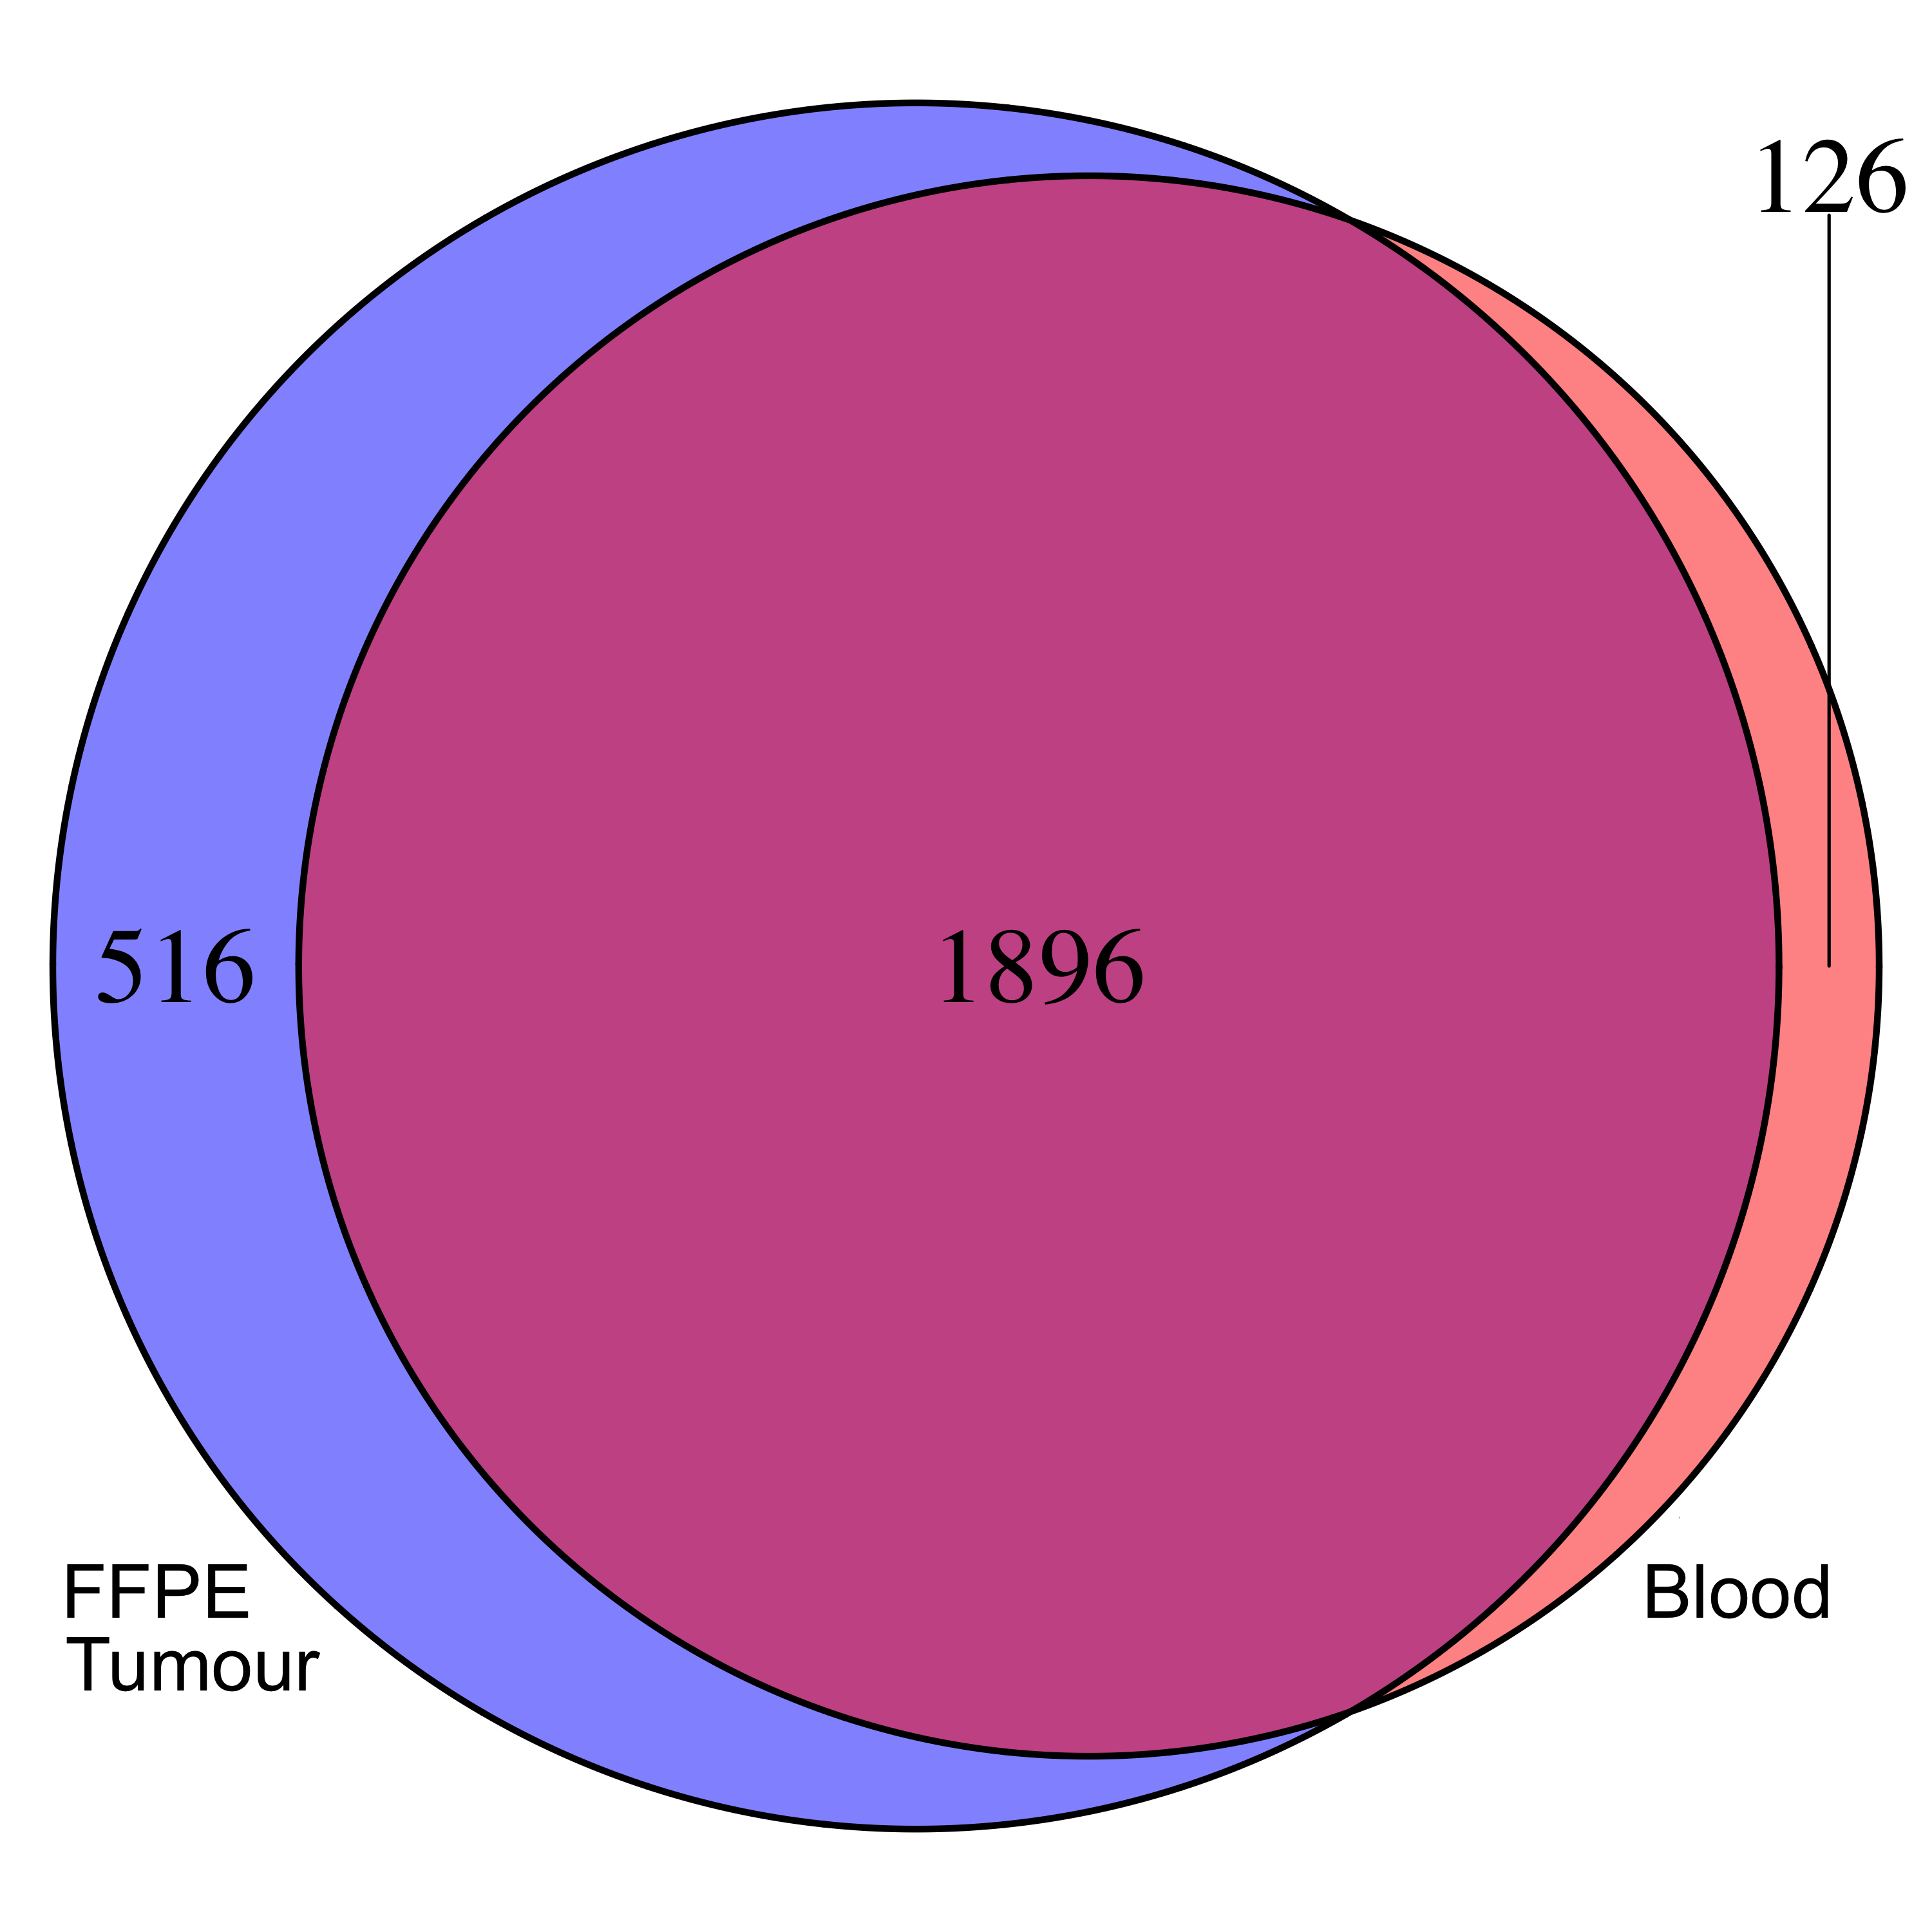
\includegraphics[scale=0.1]{ffpe_blood_conc_venn_gt.png}
	\caption{Venn diagram demonstrating concordance of variants identified in 217 tumour-blood paired samples.}
	\label{fig:ffpe_blood_conc_venn}
\end{figure}

%%%%%%%%%%%%%%%%%%%%%%%%%%%%%%%%%%%%%%%%%%%%%%%%%%%%%%%%%%%%%%%%%%%%%%
%%%%%%%%%%%%%%%%%%%%%%%%%%%%%%%%%%%%%%%%%%%%%%%%%%%%%%%%%%%%%%%%%%%%%%

\newpage
\begin{landscape}

\begin{longtable}{p{0.09\linewidth}|p{0.1\linewidth}p{0.12\linewidth}p{0.14\linewidth}p{0.17\linewidth}p{0.2\linewidth}p{0.06\linewidth}}
\caption{Distribution of discordant germline alterations identified in patients from TOP cohort.}
\label{tbl:freq_discordant_germline}
		\\
		\hline
		Gene & Chr:Pos & ID\textsuperscript{$\star$} & HGVS\textsuperscript{*} & Clinical Significance\textsuperscript{$\dagger$} & Reason for discordance & Count
		\\
		\hline
		DPYD & 1:97547947 & rs67376798 & p.Asp949Val c.2846A$>$T & Drug response & Het$/$WT & 1
		\\
		& 1:97770920 & rs1801160 & p.Val732Ile c.2194G$>$A & Benign$/$Likely benign, Not provided & Het$/$Hom & 2
		\\
		& 1:98165091 & rs2297595 & p.Met166Val c.496A$>$G & Drug response &  Het$/$Hom & 2
		\\
		& 1:98348885 & rs1801265 & p.Cys29Arg c.85T$>$C & Not provided & Low coverage in tumour & 2
		\\
		& 1:98348885 & rs1801265 & p.Cys29Arg c.85T$>$C & Not provided & Het$/$WT & 2
		\\
		& 1:98348885 & rs1801265 & p.Cys29Arg c.85T$>$C & Not provided & Het$/$Hom & 6
		\\
		\hline
		EGFR & 7:55249063 & rs1050171; COSM1451600 & p.Gln787Gln c.2361G$>$A & Benign$/$Likely benign & Het$/$Hom & 2
		\\
		\hline
		GSTP1 & 11:67352689 & rs1695 & p.Ile105Val c.313A$>$G & Drug response & Het$/$WT & 3
		\\
		& 11:67352689 & rs1695 & p.Ile105Val c.313A$>$G & Drug response & Het$/$Hom & 14
		\\
		\hline
		KIT & 4:55602765 & rs3733542; COSM1325 & p.Leu862Leu c.2586G$>$C & Benign$/$Likely benign & Het$/$Hom & 8
		\\
		\hline
		MTHFR & 1:11854476 & rs1801131 & p.Glu429Ala c.1286A$>$C & Drug response & Het$/$Hom & 12
		\\
		& 1:11856378 & rs1801133 & p.Ala222Val c.665C$>$T & Drug response & Het$/$Hom & 12
		\\
		& 1:11856378 & rs1801133 & p.Ala222Val c.665C$>$T & Drug response & Het$/$WT & 3
		\\
		\hline
		MTOR & 1:11169420 & rs41274506 & p.Asp2485Asp c.7455C$>$T & NA & Het$/$WT & 1
		\\
		& 1:11181327 & rs11121691 & p.Leu2303Leu c.6909G$>$A & NA & Het$/$Hom & 2
		\\
		& 1:11181327 & rs11121691 & p.Leu2303Leu c.6909G$>$A & NA & Low coverage in tumour & 1
		\\
		& 1:11181327 & rs11121691 & p.Leu2303Leu c.6909G$>$A & NA & Het$/$WT & 2
		\\
		& 1:11190646 & rs2275527 & p.Ser1851Ser c.5553C$>$T & Benign & Het$/$WT & 1
		\\
		& 1:11190730 & rs17848553 & p.Ala1823Ala c.5469C$>$T & Benign & Het$/$Hom & 4
		\\
		& 1:11205058 & rs1057079; rs386514433 & p.Ala1577Ala c.4731G$>$A & NA & Het$/$Hom & 8
		\\
		& 1:11205058 & rs1057079; rs386514433 & p.Ala1577Ala c.4731G$>$A & NA & Het$/$WT & 4
		\\
		& 1:1272468 & rs17036536 & p.Arg1154Arg c.3462G$>$C & Benign & Het$/$Hom & 4
		\\
		& 1:11288758 & rs1064261 & p.Asn999Asn c.2997C$>$T & NA & Het$/$Hom & 4
		\\
		& 1:11288758 & rs1064261 & p.Asn999Asn c.2997C$>$T & NA & Het$/$WT & 3
		\\
		& 1:11301714 & rs1135172 & p.Asp479Asp c.1437T$>$C & NA & Low coverage in tumour & 1
		\\
		& 1:11301714 & rs1135172 & p.Asp479Asp c.1437T$>$C & NA & Het$/$Hom & 8
		\\
		\hline
		PDGFRA & 4:55141055 & rs1873778; COSM1430082 & p.Pro567Pro c.1701A$>$G & Benign & Low coverage in tumour & 3
		\\
		& 4:55152040 & rs2228230; COSM22413 & p.Val824Val c.2472C$>$T & Benign & Het$/$WT & 2
		\\
		& 4:55152040 & rs2228230; COSM22413 & p.Val824Val c.2472C$>$T & Benign & Het$/$Hom & 4
		\\
		\hline
		STAT1 & 2:191872307 & rs45463799 & p.Asn118Asn c.354C$>$T & Likely benign & Het$/$WT & 1
		\\
		& 2:191874667 & rs386556119; rs2066802 & p.Leu21Leu c.63T$>$C & Benign & Het$/$WT & 1
		\\
		\hline
		STAT3 & 17:40498713 & NA & p.Lys49Lys c.147A$>$G & NA & Het$/$WT & 1
		\\
		\hline
		TP53 & 17:7577553 & COSM44368 & p.Met243fs c.727delA & NA & Het$/$WT & 1
		\\
		& 17:7579472 & COSM250061; rs1042522 & p.Pro72Arg c.215C$>$G & Drug response & Het$/$Hom & 26
		\\
		& 17:7579472 & COSM250061; rs1042522 & p.Pro72Arg c.215C$>$G & Drug response & Het$/$WT & 4
		\\
		& 17:7579579 & rs1800370 & p.Pro36Pro c.108G$>$A & Benign$/$Likely benign & Het$/$Hom & 2
		\\
		\hline
		TYMP & 22:50964236 & rs11479 & p.Ser471Leu c.1412C$>$T & Benign$/$Likely benign & Het$/$Hom & 14
		\\
		\hline
		TYMS & 18:673443 & rs151264360 & \footnotesize{c.*447\_*452delTTAAAG} & Drug response & Het$/$Hom & 32
		\\
		& 18:673443 & rs151264360 & \footnotesize{c.*447\_*452delTTAAAG} & Drug response & Het$/$WT & 1
		\\
		\hline
		UGT1A1 & 2:234668870 & rs873478 & c.-64G$>$C & NA & Het$/$WT & 1
		\\
		& 2:234668879 & rs34983651 & c.-55\_-54insAT & Conflicting interpretations of pathogenicity, Association & Hom$/$Het & 4
		\\
		& 2:234668879 & rs34983651 & c.-55\_-54insAT & Conflicting interpretations of pathogenicity, Association & Hom$/$WT & 2
		\\
		\hline
		\\
		&
		\multicolumn{5}{r}{Total discordant variants = 211}
		&
		\\
		\hline
\end{longtable}

%%%%%%%%%%%%%%%%%%%%%%%%%%%%%%%%%%%%%%%%%%%%%%%%%%%%%%%%%%%%%%%%%%%%%%
\noindent\textsuperscript{$\star$}dbSNP and/or COSMIC IDs.
\\
\textsuperscript{*}Description of sequence variants according to the HGVS recommendations.
\\
\textsuperscript{$\dagger$}Clinical significance on ClinVar database.
\\
Het$/$Hom = Loss of heterozygosity in the tumour
\\
Het$/$WT = Heterozygous in the blood, but wild type in the tumour
\\
Hom$/$Het = Homozygous in the blood, but heterozygous in the tumour

\end{landscape}

%%%%%%%%%%%%%%%%%%%%%%%%%%%%%%%%%%%%%%%%%%%%%%%%%%%%%%%%%%%%%%%%%%%%%%
\section{Application of tumour content to separate germline alterations from somatic mutations in tumour-only analyses}
\label{sec:Applicationoftumourcontenttoseparategermlinealterationsfromsomaticmutationsintumour-onlyanalyses}

Through variant analysis of DNA from blood specimens, we identified germline alterations that are associated with drug response, which could predict risk of developing chemotherapy-related toxicity. Furthermore, we assessed the concordance of germline variants between blood and tumour samples, which demonstrated a high concordance rate of 93.8\%. Together, these analyses confirmed that germline alterations that are clinically relevant are present in our dataset and a large proportion of germline alterations can be identified in tumour DNA with the correct designation of allelic statuses. Next, we sought to evaluate the use of variant allele frequency thresholds to separate germline alterations from somatic mutations in tumour-only analyses. Because of the lack of availability of matched normal samples in clinical genomic sequencing, this assessment would determine whether the use of variant allele frequency thresholds is an efficient approach to identify potential germline alterations in tumour-only analyses for referral to follow-up testing.

We compared the distributions of VAF of germline variants detected in blood and tumour specimens and found a significant difference between the VAF distributions of germline alterations in blood and tumour samples (Kolmogorov-Smirnov test, D = 0.17, \textit{p} = 0). As expected, we showed that heterozygous alterations in blood tend to have VAFs close to 50\%, while homozygous alterations in the blood tend to have VAFs close to 100\%. However, comparison of VAF distributions 

%%%%%%%%%%%%%%%%%%%%%%%%%%%%%%%%%%%%%%%%%%%%%%%%%%%%%%%%%%%%%%%%%%%%%%
%%%%%%%%%%%%%%%%%%%%%%%%%%%%%%%%%%%%%%%%%%%%%%%%%%%%%%%%%%%%%%%%%%%%%%

\begin{figure}[H]
	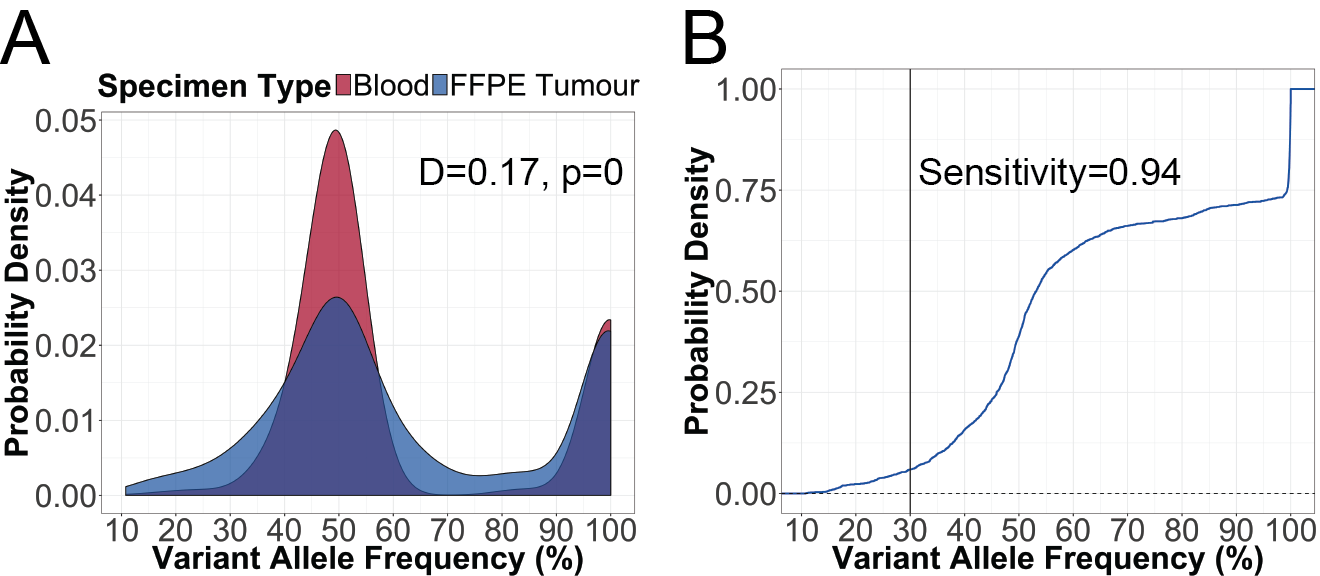
\includegraphics[scale=0.7]{germline_sens_minor.png}
	\caption{Add caption.}
	\label{fig:germline_sens_minor}
\end{figure}

%%%%%%%%%%%%%%%%%%%%%%%%%%%%%%%%%%%%%%%%%%%%%%%%%%%%%%%%%%%%%%%%%%%%%%
%%%%%%%%%%%%%%%%%%%%%%%%%%%%%%%%%%%%%%%%%%%%%%%%%%%%%%%%%%%%%%%%%%%%%%

\begin{table}[H]
\caption{Sensitivity of detecting germline variants using tumour-only analysis at various variant allele frequency thresholds.}
\label{sensitivity}
\centering
      \begin{tabular}{ccccl}
        \hline
        VAF (\%) & False Negative & True Positive & Sensitivity & 95\% CI
        \\
        \hline
        10 & 0 & 1981 & 1.0 & 1.0--1.0
        \\
        15 & 13 & 1968 & 0.99 & 0.99-1.0
        \\
        20 & 46 & 1935 & 0.98 & 0.97--0.98
        \\
        25 & 77 & 1904 & 0.96 & 0.95--0.97
        \\
        30 & 117 & 1864 & 0.94 & 0.93--0.95
        \\
        35 & 192 & 1789 & 0.90 & 0.89--0.92
        \\
        40 & 313 & 1668 & 0.84 & 0.83--0.86
        \\
        45 & 458 & 1523 & 0.77 & 0.75--0.79
        \\
				\hline
      \end{tabular} \\
\end{table}

%%%%%%%%%%%%%%%%%%%%%%%%%%%%%%%%%%%%%%%%%%%%%%%%%%%%%%%%%%%%%%%%%%%%%%
%%%%%%%%%%%%%%%%%%%%%%%%%%%%%%%%%%%%%%%%%%%%%%%%%%%%%%%%%%%%%%%%%%%%%%

\begin{figure}[H]
	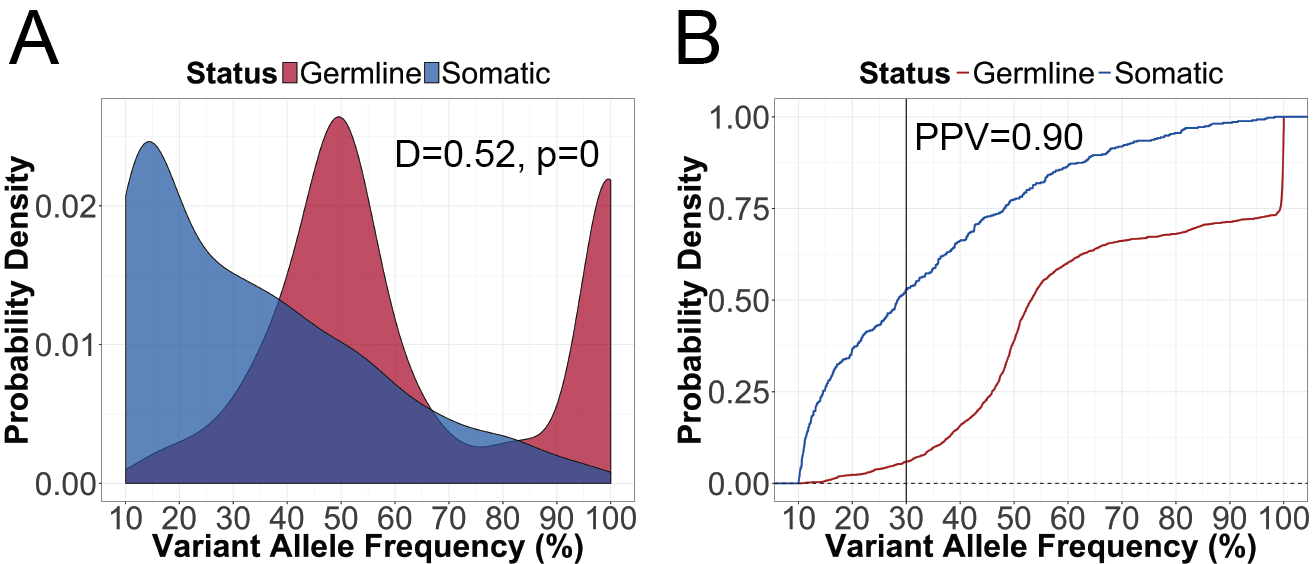
\includegraphics[scale=0.7]{germline_ppv_minor.png}
	\caption{Add caption.}
	\label{fig:germline_ppv_minor}
\end{figure}

%%%%%%%%%%%%%%%%%%%%%%%%%%%%%%%%%%%%%%%%%%%%%%%%%%%%%%%%%%%%%%%%%%%%%%
%%%%%%%%%%%%%%%%%%%%%%%%%%%%%%%%%%%%%%%%%%%%%%%%%%%%%%%%%%%%%%%%%%%%%%

\begin{table}[H]
\caption{Positive predictive value for referral of potential germline variants for downstream confirmatory testing.}
\label{ppv}
\centering
      \begin{tabular}{cccccll}
        \hline
        VAF (\%) & False Positive & True Positive & Total Calls & Positive Predictive Value & 95\% CI
        \\
        \hline
        10 & 431 & 1981 & 2412 & 0.82 & 0.81--0.84
        \\
        15 & 319 & 1968 & 2287 & 0.86 & 0.85--0.87
        \\
        20 & 273 & 1935 & 2208 & 0.88 & 0.86--0.89
        \\
        25 & 245 & 1904 & 2149 & 0.89 & 0.87--0.90
        \\
        30 & 203 & 1864 & 2067 & 0.90 & 0.89--0.91
        \\
        35 & 178 & 1789 & 1967 & 0.91 & 0.90--0.92
        \\
        40 & 146 & 1668 & 1814 & 0.92 & 0.91--0.93
        \\
        45 & 118 & 1523 & 1641 & 0.93 & 0.91--0.94
        \\
				\hline
      \end{tabular} \\
\end{table}

%%%%%%%%%%%%%%%%%%%%%%%%%%%%%%%%%%%%%%%%%%%%%%%%%%%%%%%%%%%%%%%%%%%%%%
%%%%%%%%%%%%%%%%%%%%%%%%%%%%%%%%%%%%%%%%%%%%%%%%%%%%%%%%%%%%%%%%%%%%%%


%%%%%%%%%%%%%%%%%%%%%%%%%%%%%%%%%%%%%%%%%%%%%%%%%%%%%%%%%%%%%%%%%%%%%%
\endinput
\pagebreak

\begin{table}[H]
\caption{Frequency of germline and somatic variants detected in the tumours of 213 patients in the TOP cohort.}\label{freqvariants}
\centering
\begin{tabular}{lcclcl}
        \hline
        Gene & Germline & Pathogenic Germline && Somatic \\
				 & (N Patients) & (N Patients) && (N Patients) \\
				\hline
				\\
				\multicolumn{1}{l}{\textit{Cancer predisposing}}
				&
				\multicolumn{2}{l}{ }
				&&
				\multicolumn{1}{l}{} \\
				\hline
				AKT1 & 0 & 0 && 2 (2) \\
				\arrayrulecolor{evagrey}\hline
				ALK & 1 (1) & 1 (1) && 2 (1) \\
				\hline
				BRAF & 0 & 0 && 18 (17) \\
				\hline
				EGFR & 170 (164) & 5 (5) && 31 (24) \\
				\hline
				HRAS & 0 & 0 && 1 (1) \\
				\hline
				MAP2K1 & 0 & 0 && 2 (2) \\
				\hline
				MAPK1 & 17 (17) & 3 (3) && 3 (2) \\
				\hline
				MTOR & 763 (213) & 6 (6) && 71 (30) \\
				\hline
				NRAS & 0 & 0 && 8 (8) \\
				\hline
				PDGFRA & 242 (185) & 0 && 8 (4) \\
				\hline
				PIK3CA & 0 & 0 && 15 (4) \\
				\hline
				PTEN & 0 & 0 && 1 (1) \\
				\hline
				STAT1 & 54 (51) & 1 (1) && 7 (6) \\
				\hline
				STAT3 & 10 (10) & 4 (4) && 16 (11) \\
				\hline
				TP53 & 189 (184) & 2 (2) && 131 (109) \\
				\arrayrulecolor{black}\hline
				\\
				\multicolumn{1}{l}{\textit{Pharmacogenomics}}
				&
				\multicolumn{2}{l}{ }
				&&
				\multicolumn{1}{l}{} \\
				\arrayrulecolor{black}\hline
				DPYD & 271 (212) & 1 (1) && 1 (1) \\
				\arrayrulecolor{evagrey}\hline
				GSTP1 & 106 (106) & 0 && 0 \\
				\hline
				MTHFR & 209 (177) & 0 && 0 \\
				\hline
				TYMP & 81 (76) & 2 (2) && 18 (13)\\
				\hline
				TYMS & 131 (131) & 0 && 0 \\
				\hline
				UGT1A1 & 96 (96) & 0 && 1 (1) \\
				\arrayrulecolor{black}\hline \\
				Total & 2396 (213*) & 25 (23*) && 431 (180*) \\
				\arrayrulecolor{black}\hline
      \end{tabular}
\end{table}
